% -*- latex -*-
%%%%%%%%%%%%%%%%%%%%%%%%%%%%%%%%%%%%%%%%%%%%%%%%%%%%%%%%%%%%%%%%
%%%%%%%%%%%%%%%%%%%%%%%%%%%%%%%%%%%%%%%%%%%%%%%%%%%%%%%%%%%%%%%%
%%%%
%%%% This text file is part of the source of 
%%%% `The Art of HPC, vol 4: HPC Carpentry'
%%%% by Victor Eijkhout, copyright 2012-2024
%%%%
%%%% This book is distributed under a Creative Commons Attribution 3.0
%%%% Unported (CC BY 3.0) license and made possible by funding from
%%%% The Saylor Foundation \url{http://www.saylor.org}.
%%%%
%%%%
%%%%%%%%%%%%%%%%%%%%%%%%%%%%%%%%%%%%%%%%%%%%%%%%%%%%%%%%%%%%%%%%
%%%%%%%%%%%%%%%%%%%%%%%%%%%%%%%%%%%%%%%%%%%%%%%%%%%%%%%%%%%%%%%%

\index{GNU!Make|see{Make}}
\index{Make|(}
\lstset{language=bash}

The \emph{Make} utility helps you manage the building of
projects: its main task is to facilitate rebuilding only those parts 
of a multi-file project that need to be recompiled or rebuilt.
This can save lots of time, since it
can replace a minutes-long full installation by a single file
compilation.
%% \emph{Make} can also help maintaining multiple
%% installations of a program on a single machine, for instance compiling
%% a library with more than one compiler, or compiling a program in debug
%% and optimized mode.

\emph{Make} is a Unix utility with a long history, and traditionally
there are variants with slightly different behavior, 
for instance on the various
flavors of Unix such as HP-UX, AUX, IRIX. 
These days, it is advisable, no
matter the platform, to use the GNU version of Make which has some
very powerful extensions; it is available on all Unix platforms
(on Linux it is the only available variant), and it is a {\it de
  facto} standard. The manual is available at
\url{http://www.gnu.org/software/make/manual/make.html}, or you can
read the book~\cite{OReilly-GnuMake}.

%% There are other build systems, most notably \indexterm{Scons} and
%% \indexterm{Bjam}. We will not discuss those here.
The examples in this
tutorial will be for the C and Fortran languages, but \emph{Make} can
work with any language, and in fact with things like \TeX\ that are
not really a language at all; see section~\ref{sec:latex-make}.

%%packtsnippet gnumake
\Level 0 {A simple example}

\begin{purpose}
In this section you will see a simple example, just to give the flavor of
\emph{Make}.
\end{purpose}

The files for this section can be found in the repository.

\begin{nopackt}
  \Level 1 {C++}
\end{nopackt}

Make the following files:

\ListNamedSource[C++]{foo.cxx}{tutorials/makefiles/1x}{foo.cxx}
\ListNamedSource[C++]{bar.cxx}{tutorials/makefiles/1x}{bar.cxx}
\ListNamedSource[C++]{bar.h}{tutorials/makefiles/1x}{bar.h}
and a makefile:
\ListNamedSource{Makefile}{tutorials/makefiles/1x}{Makefile}

The makefile has a number of rules like
\begin{lstlisting}
foo.o : foo.cxx
<TAB>icpc -c foo.cxx
\end{lstlisting}
which have the general form
\begin{lstlisting}
target : prerequisite(s)
<TAB>rule(s)
\end{lstlisting}
where the rule lines are indented by a \n{TAB} character.

A rule, such as above, states that a `target' file \n{foo.o} is made
from a `prerequisite' \n{foo.cxx},
namely by executing the command \n{icpc -c foo.cxx}.
(Here we are using the \indextermbus{Intel}{C++ compiler} \indextermtt{icpc};
your system could have a different compiler,
such as \indextermtt{clang++} or \indextermtt{g++}.)

The precise definition of the rule is:
\begin{itemize}
\item if the target \n{foo.o} does not exist or is older than the
  prerequisite \n{foo.cxx},
\item then the command part of the rule is executed: \n{icpc -c foo.cxx}
\item If the prerequisite is itself the target of another rule, than that
  rule is executed first.
\end{itemize}

\practical{Call \n{make}.}
  {The above rules are applied: \n{make} without arguments tries to
    build the first target, \n{fooprog}. In order to build this, it
    needs the prerequisites \n{foo.o} and \n{bar.o}, which do not
    exist. However, there are rules for making them, which \n{make}
    recursively invokes. Hence you see two compilations, for \n{foo.o}
    and \n{bar.o}, and a link command for \n{fooprog}.}
  {Typos in the makefile or in file names can cause various
    errors. In particular, make sure you use tabs and not spaces for
    the rule lines. Unfortunately, debugging a makefile is not simple. 
    \emph{Make}'s error message will usually give 
    you the line number in the make file where the error was detected.}

\practical{Do \n{make clean}, followed by \n{mv foo.cxx boo.cxx} and
  \n{make} again. Explain the error message. Restore the original file
  name.}
  {\emph{Make} will complain that there is no rule to make
    \n{foo.cxx}. This error was caused when \n{foo.cxx} was a
    prerequisite for making \n{foo.o}, and was found not to exist. 
    \emph{Make} then went
    looking for a rule to make it and no rule for creating \n{.cxx}
    files exists.}{}

Now add a second argument to the function \n{bar}.
This would require you to edit all of \n{bar.cxx}, \n{bar.h},
and \n{foo.cxx}, 
but let's say we forget to edit the last two, so only edit \n{bar.cxx}
However, it also requires you to edit \n{foo.c}, but let us for
now `forget' to do that. We will see how \emph{Make} can help you find
the resulting error.

\practical{Call \n{make} to recompile your program. Did it recompile
  \n{foo.c}?}
          {You see that inclusion of the `wrong' header file
            does not lead to an error, because C++ has polymorphism.
            In~C this would definitely give an error.
            The error only shows up in the linker stage
            because of an unresolved reference.}{}

\practical{Update the header file, and call \n{make} again. 
    What happens, and what had you been hoping would happen?}
    {Only the linker stage is done, and it gives the same error about
      an unresolved reference. Were you hoping that the main program
    would be recompiled?}

The way out of this problem is to tie the header file to the source files
in the makefile.

In the makefile, change the line
\begin{lstlisting}
foo.o : foo.cxx
\end{lstlisting}
to
\begin{lstlisting}
foo.o : foo.cxx bar.h
\end{lstlisting}
which adds \n{bar.h} as a prerequisite for \n{foo.o}. This means that,
in this case where \n{foo.o} already exists, \emph{Make} will check
that \n{foo.o} is not older than any of its prerequisites. Since
\n{bar.h} has been edited, it is younger than \n{foo.o}, so \n{foo.o}
needs to be reconstructed.

\begin{remark}
  As already noted above, in C++ fewer errors are caught by this
  mechanism than in~C, because of polymorphism.
  You might wonder if it would be possible to generate header files
  automatically. This is of course possible with suitable shell scripts,
  but tools such as \n{Make} (or~\n{CMake}) do not have this built in.
\end{remark}

\begin{nopackt}
%% remove C/F sections
  
\Level 1 {C}

Make the following files:

\ListNamedSource[C]{foo.c}{tutorials/makefiles/1c}{foo.c}
\ListNamedSource[C]{bar.c}{tutorials/makefiles/1c}{bar.c}
\ListNamedSource[C]{bar.h}{tutorials/makefiles/1c}{bar.h}
and a makefile:
\ListNamedSource{Makefile}{tutorials/makefiles/1c}{Makefile}

The makefile has a number of rules like
\begin{lstlisting}
foo.o : foo.c
<TAB>cc -c foo.c
\end{lstlisting}
which have the general form
\begin{lstlisting}
target : prerequisite(s)
<TAB>rule(s)
\end{lstlisting}
where the rule lines are indented by a \n{TAB} character.

A rule, such as above, states that a `target' file \n{foo.o} is made
from a `prerequisite' \n{foo.c}, namely by executing the command \n{cc
  -c foo.c}. The precise definition of the rule is:
\begin{itemize}
\item if the target \n{foo.o} does not exist or is older than the
  prerequisite \n{foo.c},
\item then the command part of the rule is executed: \n{cc -c foo.c}
\item If the prerequisite is itself the target of another rule, than that
  rule is executed first.
\end{itemize}

\practical{Call \n{make}.}
  {The above rules are applied: \n{make} without arguments tries to
    build the first target, \n{fooprog}. In order to build this, it
    needs the prerequisites \n{foo.o} and \n{bar.o}, which do not
    exist. However, there are rules for making them, which \n{make}
    recursively invokes. Hence you see two compilations, for \n{foo.o}
    and \n{bar.o}, and a link command for \n{fooprog}.}
  {Typos in the makefile or in file names can cause various
    errors. In particular, make sure you use tabs and not spaces for
    the rule lines. Unfortunately, debugging a makefile is not simple. 
    \emph{Make}'s error message will usually give 
    you the line number in the make file where the error was detected.}

\practical{Do \n{make clean}, followed by \n{mv foo.c boo.c} and
  \n{make} again. Explain the error message. Restore the original file
  name.}
  {\emph{Make} will complain that there is no rule to make
    \n{foo.c}. This error was caused when \n{foo.c} was a
    prerequisite for making \n{foo.o}, and was found not to exist. 
    \emph{Make} then went
    looking for a rule to make it and no rule for creating \n{.c}
    files exists.}{}

Now add a second argument to the function \n{bar}. This requires you
to edit \n{bar.c} and \n{bar.h}: go ahead and make these
edits. However, it also requires you to edit \n{foo.c}, but let us for
now `forget' to do that. We will see how \emph{Make} can help you find
the resulting error.

\practical{Call \n{make} to recompile your program. Did it recompile
  \n{foo.c}?}{Even through conceptually \n{foo.c} would need to be
  recompiled since it uses the \n{bar} function,
  \emph{Make} did not do so because the makefile had no
  rule that forced it.}{}

In the makefile, change the line
\begin{lstlisting}
foo.o : foo.c
\end{lstlisting}
to
\begin{lstlisting}
foo.o : foo.c bar.h
\end{lstlisting}
which adds \n{bar.h} as a prerequisite for \n{foo.o}. This means that,
in this case where \n{foo.o} already exists, \emph{Make} will check
that \n{foo.o} is not older than any of its prerequisites. Since
\n{bar.h} has been edited, it is younger than \n{foo.o}, so \n{foo.o}
needs to be reconstructed.

\practical{Confirm that the new makefile indeed causes \n{foo.o} to be
  recompiled if \n{bar.h} is changed. This compilation will now give
  an error, since you `forgot' to edit the use of the \n{bar} function.}{}{}

\Level 1 {Fortran}

Make the following files:

\ListNamedSource[Fortran]{foomain.F}{tutorials/makefiles/1f}{foomain.F}
\ListNamedSource[Fortran]{foomod.F}{tutorials/makefiles/1f}{foomod.F}
and a makefile:
\ListNamedSource{Makefile}{tutorials/makefiles/1f}{Makefile}
If you call \n{make}, the first rule in the makefile is executed. Do
this, and explain what happens.

\practical{Call \n{make}.}
  {The above rules are applied: \n{make} without arguments tries to
    build the first target, \n{foomain}. In order to build this, it
    needs the prerequisites \n{foomain.o} and \n{foomod.o}, which do not
    exist. However, there are rules for making them, which \n{make}
    recursively invokes. Hence you see two compilations, for \n{foomain.o}
    and \n{foomod.o}, and a link command for \n{fooprog}.}
  {Typos in the makefile or in file names can cause various
    errors. Unfortunately, debugging a makefile is not simple. You
    will just have to understand the errors, and make the
    corrections.}

\practical{Do \n{make clean}, followed by \n{mv foomod.c boomod.c} and
  \n{make} again. Explain the error message. Restore the original file
  name.}
  {\emph{Make} will complain that there is no rule to make
    \n{foomod.c}. This error was caused when \n{foomod.c} was a
    prerequisite for \n{foomod.o}, and was found not to
    exist. \emph{Make} then went looking for a rule to make it, and no
    rule for making \n{.F} files exists.}{}

Now add an extra
parameter to \n{func} in \n{foomod.F} and recompile. 

\practical{Call \n{make} to recompile your program. Did it recompile
  \n{foomain.F}?}{Even through conceptually \n{foomain.F} would need to be
  recompiled, \emph{Make} did not do so because the makefile had no
  rule that forced it.}{}

Change the line
\begin{lstlisting}
foomain.o : foomain.F
\end{lstlisting}
to
\begin{lstlisting}
foomain.o : foomain.F foomod.o
\end{lstlisting}
which adds \n{foomod.o} as a prerequisite for \n{foomain.o}. This
means that, in this case where \n{foomain.o} already exists,
\emph{Make} will check that \n{foomain.o} is not older than any of its
prerequisites. Recursively, \emph{Make} will then check if
\n{foomode.o} needs to be updated, which is indeed the case.
After recompiling \n{foomode.F}, \n{foomode.o} is younger than
\n{foomain.o}, so \n{foomain.o} will be reconstructed.

\practical{Confirm that the corrected makefile indeed causes
  \n{foomain.F} to be recompiled.}{}{}

%% end of excluded C/F section
\end{nopackt}

\Level 0 {Some general remarks}

\Level 1 {Rule interpretation}

Probably the best way to interpret a rule is:
\begin{itemize}
\item if any prerequisite has changed,
\item then the target needs to be remade,
\item and that is done by executing the commands of the rule;
\item checking the prerequisite requires a recursive application of
  make:
  \begin{itemize}
  \item if the prerequisite does not exist, find a rule to create it;
  \item if the prerequisite already exists, check applicable rules to
    see if it needs to be remade.
  \end{itemize}
\end{itemize}

\Level 1 {Make invocation}

If you call \n{make} without any arguments,
the first rule in the makefile is evaluated. You can execute other
rules by explicitly invoking them, for instance \n{make foo.o} to
compile a single file.


\Level 1 {About the make file}

The make file needs to be called \n{makefile} or
\n{Makefile}; it is not a good idea to have files with both names in
the same directory.
If you want \emph{Make} to use a different file as make file, use the
syntax \n{make -f My_Makefile}.

\Level 0 {Variables and template rules}

\begin{purpose}
  In this section you will learn various work-saving mechanisms in
  \emph{Make}, such as the use of variables and of template rules.
\end{purpose}

\Level 1 {Makefile variables}

It is convenient to introduce variables in your makefile.
For instance, 
instead of spelling out the compiler explicitly every time, introduce a
variable in the makefile:
\begin{lstlisting}
CC = gcc
FC = gfortran
\end{lstlisting}
and use \verb+${CC}+ or \verb+${FC}+ on the compile lines:
\begin{lstlisting}
foo.o : foo.c
        ${CC} -c foo.c
foomain.o : foomain.F
        ${FC} -c foomain.F
\end{lstlisting}
\practical{Edit your makefile as indicated. First do \n{make clean},
  then \n{make foo} (C) or \n{make fooprog} (Fortran).}
  {You should see the exact same compile and link lines as before.}
  {Unlike in the shell, where braces are optional, variable names in a
    makefile have to be in
    braces or parentheses. Experiment with what happens if you forget
    the braces around a variable name.}

One
advantage of using variables is that you can now change the compiler
from the commandline:
\begin{lstlisting}
make CC="icc -O2"
make FC="gfortran -g"
\end{lstlisting}

\practical{Invoke \emph{Make} as suggested (after \n{make clean}). Do
  you see the difference in your screen output?}
  {The compile lines now show the added compiler option \n{-O2} or \n{-g}.}{}

\emph{Make} also has \emph{automatic variables}\index{Make!automatic variables|textbf}:
\begin{itemize}
\item [\n{\$@}] The target. Use this in the link line for the main
  program. % (See section \ref{sec:target-prereq} for some trickery
  % with~\verb+$@+.)
\item [\n{\$\char`\^}] The list of prerequisites. Use this also in the link
  line for the program.
\item [\n{\$<}] The first prerequisite. Use this in the compile
  commands for the individual object files.
\item [\n{\$*}] In \emph{template rules}\index{Make!template rules}
  (section~\ref{sec:make-template}) this matches the template part,
  the part corresponding to the~\n{\char37}.
\end{itemize}
Using these variables, the rule for \n{fooprog} becomes
\begin{lstlisting}
fooprog : foo.o bar.o
        ${CC} -o $@ $^
\end{lstlisting}
and a typical compile line becomes
\begin{lstlisting}
foo.o : foo.c bar.h
        ${CC} -c $<
\end{lstlisting}

You can also declare a variable
\begin{lstlisting}
THEPROGRAM = fooprog
\end{lstlisting}
and use this variable instead of the program name in your
makefile. This makes it easier to change your mind about the name of
the executable later. 

\practical{Edit your makefile to add this variable definition, and use
  it instead of the literal program name. Construct a commandline so
  that your makefile will build the executable \n{fooprog\_v2}.}{You
  need to specify the \n{THEPROGRAM} variable on the commandline using
  the syntax \n{make VAR=value}.}  {Make sure that there are no spaces
  around the equals sign in your commandline.}

The full list of these automatic variables can be found at
\url{https://www.gnu.org/software/make/manual/html_node/Automatic-Variables.html}.

\Level 1 {Template rules}
\label{sec:make-template}
\index{template rule|see{Make, template rule}}

So far, you wrote a separate rule for each file that
needed to be compiled. However, the rules for the various \n{.c}
files are very similar:
\begin{itemize}
\item the rule header (\n{foo.o : foo.c}) states that a source file is a
  prerequisite for the object file with the same base name;
\item and the instructions for compiling (\n{\$\{CC\} -c \$<}) 
  are even character-for-character the
  same, now that you are using \emph{Make}'s built-in variables;
\item the only rule with a difference is 
\begin{lstlisting}
foo.o : foo.c bar.h
        ${CC} -c $<
\end{lstlisting}
  where the object file depends on the source file and another file.
\end{itemize}
We can take the commonalities and summarize them in one 
\emph{template rule}\index{Make!template rules}\footnote
{This mechanism is the first instance you'll see that only exists in
  GNU make, though in this particular case there is a similar
  mechanism in standard make. That will not be the case for the
  wildcard mechanism in the next section.}:
\begin{lstlisting}
%.o : %.c
        ${CC} -c $<
%.o : %.F
        ${FC} -c $<
\end{lstlisting}
This states that any object file depends on the C or Fortran file with
the same base name. To regenerate the object file, invoke the C or
Fortran compiler with the \n{-c} flag.
These template rules can function as a replacement for the multiple
specific targets in the makefiles above, except for the rule for \n{foo.o}.

The dependence of \n{foo.o} on \n{bar.h}, or \n{foomain.o} on
\n{foomod.o}, can be handled by adding a rule
\begin{lstlisting}
# C
foo.o : bar.h
# Fortran
foomain.o : foomod.o
\end{lstlisting}
with no further instructions. This rule states, `if file
\n{bar.h} or \n{foomod.o} changed, file \n{foo.o} or \n{foomain.o}
needs updating' too. \emph{Make} will
then search the makefile for a different
rule that states how this updating is done, and it will find the
template rule.

\practical{Change your makefile to incorporate these ideas, and test.}{}{}

\begin{figure}[ht]
  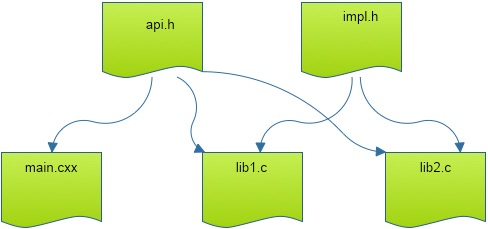
\includegraphics[scale=.5]{make-exercises}
  \caption{File structure with main program and two library files.}
  \label{fig:make-exercises}
\end{figure}

\begin{figure}[t]
  \begin{multicols}{2}
    Source file \n{mainprog.cxx}:
    \ListStrippedSource{code/make}{mainprog.cxx}
    Source file \n{libf.cxx}:
    \ListStrippedSource{code/make}{libf.cxx}
    Source file \n{libg.cxx}:
    \ListStrippedSource{code/make}{libg.cxx}
    Header file \n{api.h}:
    \ListStrippedSource{code/make}{api.h}
    Header file \n{impl.h}:
    \ListStrippedSource{code/make}{impl.h}
  \end{multicols}
  \caption{Source files for exercise~\ref{ex:make-main-lib}.}
  \label{fig:make-files}
\end{figure}

\begin{exercise}
  \label{ex:make-main-lib}
  Write a makefile for the following structure:
  \begin{itemize}
  \item There is one main file \n{libmain.cxx}, and two library files
    \n{libf.cxx} \n{libg.cxx};
  \item There is a header file \n{libapi.h} that gives the prototypes
    for the functions in the library files;
  \item There is a header file \n{libimpl.h} that gives implementation
    details, only to be used in the library files.
  \end{itemize}
  This is illustrated in figure~\ref{fig:make-exercises}.

  Here is how you can test it:
  \begin{multicols}{2}
    \footnotesize
    Changing a source file only recompiles that files:
\begin{lstlisting}
clang++ -c libf.cxx
clang++ -o main \
    libmain.o libf.o libg.o
\end{lstlisting}
Changing the implementation header only recompiles the library:
\begin{lstlisting}
clang++ -c libf.cxx
clang++ -c libg.cxx
clang++ -o main libmain.o libf.o libg.o  
\end{lstlisting}
Changing the \n{libapi.h} recompiles everything:
\begin{lstlisting}
clang++ -c libmain.cxx
clang++ -c libf.cxx
clang++ -c libg.cxx
clang++ -o main libmain.o libf.o libg.o
\end{lstlisting}
  \end{multicols}
\end{exercise}

\begin{figure}[ht]
  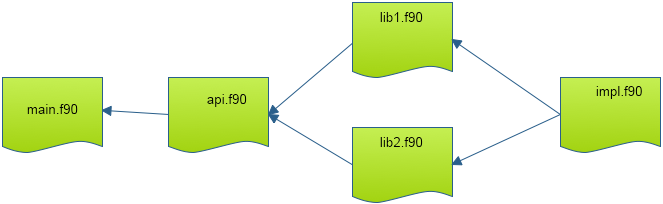
\includegraphics[scale=.5]{make-exercises-f}
  \caption{File structure with main program and two library files.}
  \label{fig:make-exercises-f}
\end{figure}

\begin{nopackt}
For Fortran we don't have header files so
we use \emph{modules}\index{Fortran!module}
everywhere; figure~\ref{fig:make-exercises-f}.
If you know how to use
\emph{submodules}\index{Fortran!submodule},
a \indexterm{Fortran2008} feature,
you can make the next exercise as efficient
as the C version.
\index{module|see{Fortran, module}}

\begin{exercise}
  \label{ex:make-main-lib-f}
  Write a makefile for the following structure:
  \begin{itemize}
  \item There is one main file \n{libmain.f90},
    that uses a module \n{api.f90};
  \item There are two low level modules \n{libf.f90} \n{libg.f90}
    that are used in \n{api.f90}.
  \end{itemize}
  If you use modules,
  you'll likely be doing more compilation than needed.
  For the optimal solution,
  use submodules.
\end{exercise}
\end{nopackt}

\Level 1 {Wildcards}

Your makefile now uses one general rule for compiling any source
file. Often, your source files will be all the \n{.c} or \n{.F}
files in your directory, so is there a way to state `compile
everything in this directory'? Indeed there is.


Add the following lines
to your makefile, and use the variable \n{COBJECTS} or \n{FOBJECTS}
wherever appropriate.
The command \indextermtt{wildcard} gives the result of \n{ls},
and you can manipulate file names with \indextermtt{patsubst}.
\begin{lstlisting}
# wildcard: find all files that match a pattern
CSOURCES := ${wildcard *.c}
# pattern substitution: replace one pattern string by another
COBJECTS := ${patsubst %.c,%.o,${SRC}}

FSOURCES := ${wildcard *.F}
FOBJECTS := ${patsubst %.F,%.o,${SRC}}
\end{lstlisting}

\Level 1 {More functions}

GNU make has more function that you can call inside the makefile.
Some examples:
\begin{lstlisting}
HOSTNAME := $(shell hostname -f)
SOURCES  := $(wildcard *.c)
OBJECTS  := $(patsubst %.c,%.o,${SOURCES})
RECURSIVE := $(foreach d,${DIRECTORIES},$(wildcard ${d}/*.c))
\end{lstlisting}
File name manipulation:
\begin{lstlisting}
$(dir a/b/c.x)    # gives `a/b'
$(dir c.x)        # gives `./'
$(notdir a/b/c.x) # gives `c.x'
$(suffix a/b/c.x) # gives `.x'
\end{lstlisting}
For the full list see \url{https://www.gnu.org/software/make/manual/html_node/Functions.html}.

\begin{multicols}{2}
  \lstinputlisting{snippets/makerulesrc}
  \columnbreak
  \lstinputlisting{snippets/makeout-src}
\end{multicols}
\begin{multicols}{2}
  \lstinputlisting{snippets/makeruleobj}
  \columnbreak
  \lstinputlisting{snippets/makeout-obj}
\end{multicols}
\begin{multicols}{2}
  \lstinputlisting{snippets/makerulepre}
  \columnbreak
  \lstinputlisting{snippets/makeout-pre}
\end{multicols}
\begin{multicols}{2}
  \lstinputlisting{snippets/makerulebak}
  \columnbreak
  \lstinputlisting{snippets/makeout-bak}
\end{multicols}

\Level 1 {Conditionals}

There are various ways of making the behavior of a makefile dynamic.
You can for instance put a shell conditional in an action line.
However, this can make for a cluttered makefile; an easier way is to use
makefile conditionals. There are two types of conditionals: tests on string
equality, and tests on environment variables.

The first type looks like
\begin{lstlisting}
ifeq "${HOME}" "/home/thisisme"
  # case where the executing user is me
else ifeq "${HOME}" "/home/buddyofmine"
  # case for other user 
else
  # case where it's someone else
endif
\end{lstlisting}
and in the second case the test looks like
\begin{lstlisting}
ifdef SOME_VARIABLE
\end{lstlisting}
The text in the true and false part can be most any part of a
makefile. For instance, it is possible to let one of the action lines
in a rule be conditionally included. However, most of the times you
will use conditionals to make the definition of variables dependent on
some condition.

\practical{Let's say you want to use your makefile at home and at
  work. At work, your employer has a paid license to the Intel
  compiler \n{icc}, but at home you use the open source Gnu compiler
  \n{gcc}. Write a makefile that will work in both places, setting the
  appropriate value for \n{CC}.}{}{}

\Level 0 {Miscellania}

\Level 1 {Phony targets}

The example makefile contained a target \n{clean}. This uses
the \emph{Make} mechanisms to accomplish some actions that are not
related to file creation: calling \n{make clean} causes \emph{Make} to
reason `there is no file called \n{clean}, so the following
instructions need to be performed'. However, this does not actually
cause a file \n{clean} to spring into being, so calling \n{make clean}
again will make the same instructions being executed.

To indicate that this rule does not actually make the target, you use
the \indextermtt{.PHONY} keyword:
\begin{lstlisting}
.PHONY : clean
\end{lstlisting}
Most of the time, the makefile will actually work fine without this
declaration, but the main benefit of declaring a target to be phony is
that the \emph{Make} rule will still work, even if you have a file (or folder)
named \n{clean}.

\Level 1 {Directories}

It's a common strategy to have a directory for temporary material
such as object files. So you would have a rule
\begin{lstlisting}
obj/%.o : %.c
    ${CC} -c $< -o $@
\end{lstlisting}
and to remove the temporaries:
\begin{lstlisting}
clean ::
    rm -rf obj
\end{lstlisting}
This raises the question how the \n{obj} directory is created.
You could do:
\begin{lstlisting}
obj/%.o : %.c
    mkdir -p obj
    ${CC} -c $< -o $@
\end{lstlisting}
but a better solution is to use
\indextermsub{order-only}{prerequisite}s exist.
\begin{lstlisting}
obj :
    mkdir -p obj
obj/%.o : %.c | obj
    ${CC} -c $< -o $@
\end{lstlisting}
This only tests for the existence of the object directory,
but not its timestamp.

\Level 1 {Using the target as prerequisite}

Suppose you have two different targets that are treated largely the
same. You would want to write:
\begin{lstlisting}
PROGS = myfoo other
${PROGS} : $@.o # this is wrong!!
        ${CC} -o $@ $@.o ${list of libraries goes here}
\end{lstlisting}
and saying \n{make myfoo} would cause 
\begin{lstlisting}
cc -c myfoo.c
cc -o myfoo myfoo.o ${list of libraries}
\end{lstlisting}
and likewise for \n{make other}. What goes wrong here is the use of
\verb+$@.o+ as prerequisite. In Gnu Make, you can repair this as
follows\footnote{Technical explanation: Make will now look at lines
  twice: the first time \n{\$\$} gets converted to a single~\n{\$},
  and in the second pass \n{\$@} becomes the name of the target.}:
\begin{lstlisting}
.SECONDEXPANSION:
${PROGS} : $$@.o
        ${CC} -o $@ $@.o ${list of libraries goes here}
\end{lstlisting}

\practical{Write a second main program \n{foosecond.c} or
  \n{foosecond.F}, and change your makefile so that the calls
  \n{make foo} and \n{make foosecond} both use the same rule.}{}{}

\Level 1 {Predefined variables and rules}

Calling \n{make -p yourtarget} causes make to print out all its
actions, as well as the values of all variables and rules, both in
your makefile and ones that are predefined. If you do this in a
directory where there is no makefile, you'll see that make actually
already knows how to compile \n{.c} or \n{.F} files. Find this rule
and find the definition of the variables in it.

You see that you can customize make by setting such variables as
\n{CFLAGS} or \n{FFLAGS}. Confirm this with some experimentation. If
you want to make a second makefile for the same sources, you can call
\n{make -f othermakefile} to use this instead of the default
\n{Makefile}.

Note, by the way, that both \n{makefile} and \n{Makefile} are
legitimate names for the default makefile. It is not a good idea to
have both \n{makefile} and \n{Makefile} in your directory.

\Level 0 {Shell scripting in a Makefile}
\label{sec:make-shell}

\begin{purpose}
  In this section you will see an example of a longer shell script
  appearing in a makefile rule.
\end{purpose}

In the makefiles you have seen so far, the command part was a single
line. You can actually have as many lines there as you want.
For example, let us make a rule for making backups of the program you
are building.

Add a \n{backup}  rule to your makefile. The first thing it needs to
do is make a backup directory:
\begin{lstlisting}
.PHONY : backup
backup :
        if [ ! -d backup ] ; then 
          mkdir backup
        fi
\end{lstlisting}
Did you type this? Unfortunately it does not work: every line in the
command part of a makefile rule gets executed as a single
program. Therefore, you need to write the whole command on one line:
\begin{lstlisting}
backup :
        if [ ! -d backup ] ; then mkdir backup ; fi
\end{lstlisting}
or if the line gets too long:
\begin{lstlisting}
backup :
        if [ ! -d backup ] ; then \
          mkdir backup ; \
        fi
\end{lstlisting}
(Writing a long command on a single is only possible
in the \indextermunix{bash} shell, not in the \indextermunix{csh} shell.
This is one reason for not using the latter.)

Next we do the actual copy:
\begin{lstlisting}
backup :
        if [ ! -d backup ] ; then mkdir backup ; fi
        cp myprog backup/myprog
\end{lstlisting}
But this backup scheme only saves one version. Let us make a version
that has the date in the name of the saved program. 

The Unix \n{date} command can customize its output by accepting a
format string. Type the following: 
%
\verb+date +%Y%m%d+. 
%
This can be used in the makefile.

\begin{nopackt}
\practical {Edit the {\tt cp} command line so that the name of the
  backup file includes the current date.}{Hint: you need the
  backquote.
  Consult the Unix tutorial, section~\ref{tut:unix-bq}, if
  you do not remember what backquotes do.
}{}
\end{nopackt}

If you are defining shell variables in the command section of a
makefile rule, you need to be aware of the following. Extend your
\n{backup} rule with a loop to copy the object files:
\begin{lstlisting}
#### This Script Has An ERROR!
backup :
        if [ ! -d backup ] ; then mkdir backup ; fi
        cp myprog backup/myprog
        for f in ${OBJS} ; do \
          cp $f backup ; \
        done
\end{lstlisting}
(This is not the best way to copy, but we use it for the purpose of
demonstration.) This leads to an error message, caused by the fact
that \emph{Make} interprets \verb+$f+ as an environment variable of
the outer process. What works is:
\begin{lstlisting}
backup :
        if [ ! -d backup ] ; then mkdir backup ; fi
        cp myprog backup/myprog
        for f in ${OBJS} ; do \
          cp $$f backup ; \
        done
\end{lstlisting}
(In this case \emph{Make} replaces the double dollar by a single one
when it scans the commandline. During the execution of the
commandline, \n{\$f} then expands to the proper filename.)

\Level 0 {Practical tips for using Make}
Here are a couple of practical tips.

\begin{itemize}
\item \emph{Debugging}\index{Make!debugging} a makefile is often
  frustratingly hard.  Just about the only tool is the \n{-p} option,
  which prints out all the rules that Make is using, based on the
  current makefile.
\item You will often find yourself first typing a make command, and
  then invoking the program. Most Unix shells allow you to use
  commands from the \indextermbus{shell}{command history} by using the
  up arrow key. Still, this may get tiresome, so you may be tempted to
  write
\begin{lstlisting}
make myprogram ; ./myprogram -options
\end{lstlisting}
and keep repeating this.
There is a danger in this: if the make fails, for instance because of
compilation problems, your program will still be executed. Instead, write
\begin{lstlisting}
make myprogram && ./myprogram -options
\end{lstlisting}
which executes the program conditional upon make concluding successfully.
\end{itemize}

\Level 1 {What does this makefile do?}

Above you learned that issuing the \n{make} command will automatically
execute the first rule in the makefile. This is convenient in one
sense\footnote {There is a convention among software developers that a
  package can be installed by the sequence \n{./configure ; make ;
    make install}, meaning: Configure the build process for this
  computer, Do the actual build, Copy files to some system directory
  such as \n{/usr/bin}.}, and inconvenient in another: the only way to
find out what possible actions a makefile allows is to read the
makefile itself, or the --~usually insufficient~-- documentation.

A better idea is to start the makefile with a target
\begin{lstlisting}
info :
        @echo "The following are possible:"
        @echo "  make"
        @echo "  make clean"
\end{lstlisting}
Now \n{make} without explicit targets informs you of the capabilities
of the makefile.

If your makefile gets longer, you might want to document each section
like this. This runs into a problem: you can not have two rules with the same
target, \n{info} in this case. However, if you use a double colon
it \emph{is} possible. Your makefile would have the following structure:
\begin{lstlisting}
info ::
        @echo "The following target are available:"
        @echo "  make install"
install :
        # ..... instructions for installing
info ::
       @echo "  make clean"
clean :
       # ..... instructions for cleaning
\end{lstlisting}

\Level 0 {A Makefile for \LaTeX}
\label{sec:latex-make}
\index{Make!and LaTeX@{and \LaTeX}|(}

The \emph{Make} utility is typically used for compiling programs, but
other uses are possible too. In this section, we will discuss a
makefile for \LaTeX\ documents.

We start with a very basic makefile:
\lstinputlisting{tutorials/makefiles/tex/M0}
The command \n{make myfile.pdf} will invoke \n{pdflatex myfile.tex},
if needed, once. Next we repeat invoking \n{pdflatex} until the log file no
longer reports that further runs are needed:
\lstinputlisting{tutorials/makefiles/tex/M1}
We use the \verb+${basename fn}+ macro to extract the base name
without extension from the target name.

In case the document has a bibliography or index, we run \n{bibtex}
and \n{makeindex}. 
\lstinputlisting{tutorials/makefiles/tex/M2}
The minus sign at the start of the line means that
\emph{Make} should not exit if these commands fail.

Finally, we would like to use \emph{Make}'s facility for taking
dependencies into account. 
We could write a makefile that has
the usual rules
\begin{lstlisting}
mainfile.pdf : mainfile.tex includefile.tex
\end{lstlisting}
but we can also discover the include files explicitly. The following
makefile is invoked with 
\begin{lstlisting}
  make pdf TEXTFILE=mainfile
\end{lstlisting}
The \n{pdf} rule then uses some shell scripting to discover the
include files (but not recursively), and it calls \emph{Make} again,
invoking another rule, and passing the dependencies explicitly.
\lstinputlisting{tutorials/makefiles/tex/Makefile}
This shell scripting can also be done outside the makefile, generating
the makefile dynamically.

\index{Make!and LaTeX@{and \LaTeX}|)}
\index{Make|)}

\endinput

\Level 0 {Cmake}
\index{Cmake|(textbf}

Makefiles can be cumbersome to make, and they may need customization
for any specific installation. For this reason, \emph{Cmake} is a
build system that first generates the makefiles, which can then be
used in the normal manner.

Here are the main components:
\begin{itemize}
\item The source directory has a file \indextermtt{CMakeLists.txt}
  that describes the structure of the application.
\item Generated files can be kept separate from the source:
\begin{lstlisting}
sourcedir=.... # source location
builddir=....  # place for temporaries
installdir=... # here goes the finished stuff
cd ${builddir}
cmake \
  -DCMAKE_PREFIX_PATH=${installdir} \
  ${sourcedir} # do the setup
make           # compile
make install   # move finished stuff in place
\end{lstlisting}
\end{itemize}

\Level 1 {Dependency analysis}

Above you learned how \n{Make} can be used for projects with
complicated dependencies. You can tell \n{Cmake} about this using
clauses
\begin{lstlisting}
include_directories(include)
file(GLOB SOURCES "*/*.c")
file(GLOB HEADERS "*/*.h")
add_executable(hello_world hello.c ${SOURCES} )
\end{lstlisting}
%%%% VLE this seems to be old style. should not use `include_directories'
When invoked, \n{Cmake} will then report
\begin{lstlisting}
Scanning dependencies of target hello_world
\end{lstlisting}
and generate makefiles accordingly.

One advantage of this setup is that the \n{cmake} stage only needs to
be redone if the structure of the application changes, for instance
because files are added. For any ordinary edits during program
development it is enough to repeat the \n{make} and \n{make install}
part.

Example. Consider a main file \n{hello.c} that uses two auxiliary
files \n{compute.c} and \n{output.c}. After cmake, the \n{make; make
  install} gives as output:
\begin{lstlisting}
Scanning dependencies of target hello_world
[ 25%] Building C object CMakeFiles/hello_world.dir/hello.c.o
[ 50%] Building C object
                CMakeFiles/hello_world.dir/compute/compute.c.o
[ 75%] Building C object CMakeFiles/hello_world.dir/output/output.c.o
[100%] Linking C executable hello_world
[100%] Built target hello_world
[100%] Built target hello_world
Install the project...
\end{lstlisting}
After editing the \n{compute.c} file only that is recompiled, and the
project is relinked:
\begin{lstlisting}
Scanning dependencies of target hello_world
[ 25%] Building C object
                
CMakeFiles/hello_world.dir/compute/compute.c.o
[100%] Built target hello_world
[100%] Built target hello_world
Install the project...
\end{lstlisting}
Clearly, cmake has generated makefiles with the right structure.
The disadvantage of using \n{cmake} is that the automatically
generated makefiles are close to unreadable.

\Level 1 {Re-Cmaking}

The structure sketched just now, with a separate build and install
directory, means that completely deleting these libraries is enough to
start with a clean slate. For a more modest approach, you can delete
the file \indextermtt{CMakeCache.txt}, which is in the build directory.

\Level 1 {System dependencies}

You can give \n{Cmake} options that find their way into the makefile
structure. For instance, on the Apple laptop where this book was
written, a straight invocation make \n{Cmake} discover the C~compiler of the system:
\begin{lstlisting}
-- The C compiler identification is AppleClang 9.1.0.9020039
\end{lstlisting}
However, specifying
\begin{lstlisting}
cmake -DCMAKE_C_COMPILER=gcc
\end{lstlisting}
gives:
\begin{lstlisting}
-- The C compiler identification is GNU 7.4.0
\end{lstlisting}

\Level 1 {Details}

CMake has variables:
\begin{lstlisting}
set(myvar myvalue)
message(STATUS "my variable has value ${myvar}")
\end{lstlisting}
\index{Cmake|)}

%%packtsnippet end

% LocalWords:  Eijkhout
